\subsection{Simulation and Simplified Model}
The previous sections show a velocity model of the system which is modelled in this section. As mentioned in the inertia test, \appref{app:inertiaTest}, the armature inductance is so small that it is not necessary to include for a good simulation. If the armature inductance is neglectable, and removed, the system will appear as a first order system instead of a second order. Therefore \si{L_a} is set to zero and hence removing the second order term. This effect is illustrated in the transfer function:
%
\begin{flalign}
  \eq{\frac{V(s)}{U_a(s)}}{ \frac{K_t}{L_a \cdot J_{tot} \cdot s^2 + (R_a \cdot J_{tot} + L_a \cdot B_{tot}) \cdot s + R_a \cdot B_{tot} + K_t \cdot K_e }}\nonumber\\
  &\Downarrow&\nonumber\\
  \eq{\frac{V(s)}{U_a(s)}}{ \frac{ K_t }{ R_a \cdot J_{tot}  \cdot s + R_a \cdot B_{tot} + K_t \cdot K_e }}\nonumber\\
  \eq{\frac{V(s)}{U_a(s)}}{ \frac{ \frac{K_t}{R_a \cdot B_{tot} + K_t\cdot K_e} }{ \frac{R_a \cdot J_{tot}}{R_a \cdot B_{tot} + K_t \cdot K_e}\cdot s + 1 }}
  \label{eq:simplifiedTransferVel}
\end{flalign}
%
By inspection of the first order expression, in \eqref{eq:simplifiedTransferVel}, the terms for the time constant and the gain are extracted:
\begin{flalign}
  \eq{K}{\frac{K_t}{R_a \cdot B_{tot} + K_t\cdot K_e}}&\nonumber\\
  \eq{\tau }{ \frac{R_a \cdot J}{R_a \cdot B_{tot} + K_t \cdot K_e} }\nonumber&
\end{flalign}
%
To verify that this is a viable approximation, the following simplified model, in \figref{fig:BlockDiagramDrivetrainSimplified}, is created:
%
\begin{figure}[H]
	\centering
	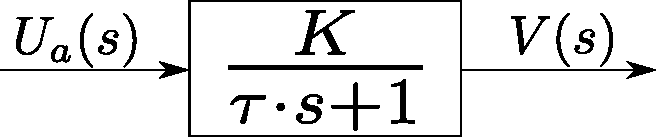
\includegraphics[scale = .5]{figures/totalVelocityModelDiagramSimplified.pdf}
	\caption{A block diagram showing a simplified model}
	\label{fig:BlockDiagramDrivetrainSimplified}
\end{figure}
%
Where \si{K} is the gain of the system and \si{\tau} is the time constant. This simplified first order model of the system is simulated alongside the second order model, to verify that the vehicle can indeed be handled as a first order system. The plot of the two simulations are illustrated in \figref{fig:ComparisonOf1stAnd2ndOrderModels}.
%
\begin{figure}[H]
	\centering
	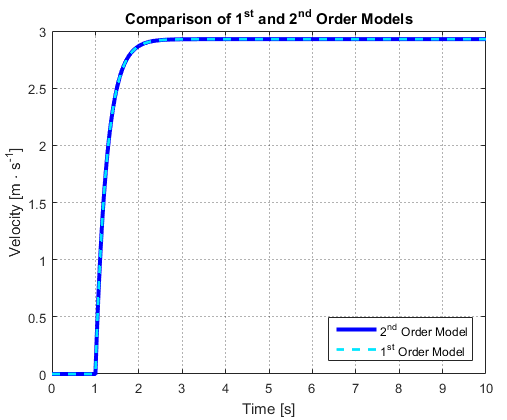
\includegraphics[width = .8\textwidth]{figures/ComparisonOf1stAnd2ndOrderModels.png}
	\caption{Comparison of the \si{1^{st}} and \si{2^{nd}} order models}
	\label{fig:ComparisonOf1stAnd2ndOrderModels}
\end{figure}
%
\todo{Change picture}

In the following section the simplified model is verified directly by comparison with recorded data of the vehicle's step response.